\chapter{微积分基本定理和场论}

本章介绍多元函数积分的三个重要公式,Green公式、Gauss公式和Stokes公式,及梯度、散度和旋度。
这三个公式是物理的基本公式,可以认为是多元函数微积分在物理方面的基础,是前几章在物理方面的应用。

本章要点:
\begin{itemize}
    \item Green公式。
    \item Gauss公式。
    \item Stokes公式。
    \item 保守场。
    \item 微积分基本定理。
\end{itemize}

~

\newpage
\section{格林Green公式}

本节讨论格林Green公式。
Green公式是二维平面的二重积分和边界积分的关系,是后续两个公式的“预热”。

本节要点:
\begin{itemize}
    \item 掌握Green公式的概念。
\end{itemize}

%============================================================
\subsection{格林Green公式的概念}

\begin{definition}[Green公式]
假设二维平面中有单连通区域$D$,其正向边界$L$分段光滑,$\boldsymbol{f}\left( \boldsymbol{p} \right) =\left( P\,\,Q \right) ^T$是定义在二维平面上的向量值函数,且$P,Q$在$D$上有一阶连续偏导数,则有:
\[
\oint\limits_L{\boldsymbol{f}^T\boldsymbol{dl}}=\oint\limits_L{Pdx+Qdy}=\iint\limits_D{\left( \frac{\partial Q}{\partial x}-\frac{\partial P}{\partial y} \right) dxdy}
\]
上述公式称为{\bf Green公式}。
若假设$D$为复连通区域,其正向外边界为$L_1$,正向内边界为$L_2$,则有:
\[
\oint\limits_{L_1}{\boldsymbol{f}^T\boldsymbol{dl}}+\oint\limits_{L_2}{\boldsymbol{f}^T\boldsymbol{dl}}=\iint\limits_D{\left( \frac{\partial Q}{\partial x}-\frac{\partial P}{\partial y} \right) dxdy}
\]
\end{definition}

\begin{figure}[h]
\centering
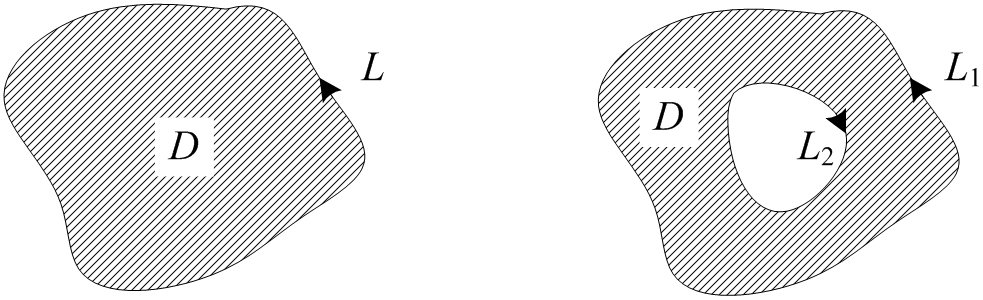
\includegraphics[height=2.5cm]{11.1.png}
\end{figure}






\newpage
\section{高斯Gauss公式和散度}

本节介绍Gauss公式。

本节要点:
\begin{itemize}
    \item 掌握Gauss公式的概念;
    \item 理解Gauss公式的物理意义;
    \item 掌握散度的概念;
    \item 理解散度的物理意义。
\end{itemize}

%============================================================
\subsection{Gauss公式的概念}

\begin{definition}[Gauss公式]
假设三维空间中有单连通区域$V$,其外侧边界$S$分片光滑,$\boldsymbol{f}\left( \boldsymbol{p} \right) =\left( P\,\,Q\,\,R \right) ^T$是定义在三维空间上的向量值函数,且$P,Q,R$在$V$上有一阶连续偏导数,则有:
\begin{align*}
&\oiint\limits_S{\boldsymbol{f}^T\boldsymbol{ds}}=\oiint\limits_S{Pdydz+Qdzdx+Rdxdy}= \\
&\iiint\limits_V{\left( \frac{\partial P}{\partial x}+\frac{\partial Q}{\partial y}+\frac{\partial R}{\partial z} \right) dv}
\end{align*}
上述公式称为{\bf Gauss公式}。
\end{definition}

%============================================================
\subsection{Gauss公式的物理意义}

Gauss公式左边代表一个矢量场对于一个封闭曲面的总通量:
\begin{itemize}
    \item $\boldsymbol{f}^T\boldsymbol{ds}$:通量微元,或者说是矢量场在曲面微元形成的通量;
    \item $\oiint_S$:对整个封闭曲面的总累积量;
    \item $\oiint_S{\boldsymbol{f}^T\boldsymbol{ds}}=0$:通量为0,表示流入流出该空间的量相抵消;
    \item $\oiint_S{\boldsymbol{f}^T\boldsymbol{ds}}>0$:表示有东西流出该区域;
    \item $\oiint_S{\boldsymbol{f}^T\boldsymbol{ds}}<0$:表示有东西流入该区域。
\end{itemize}

Gauss公式右边代表这个封闭曲面中源或者汇:
\begin{itemize}
    \item $\left( \frac{\partial P}{\partial x}+\frac{\partial Q}{\partial y}+\frac{\partial R}{\partial z} \right) dv$:该点处的源或者汇;
    \item $\iiint_V$:整个区域中的所有的源或汇;
    \item $\iiint_V{\left( \frac{\partial P}{\partial x}+\frac{\partial Q}{\partial y}+\frac{\partial R}{\partial z} \right) dv}=0$:表示区域内既无源也无汇;
    \item $\iiint_V{\left( \frac{\partial P}{\partial x}+\frac{\partial Q}{\partial y}+\frac{\partial R}{\partial z} \right) dv}>0$:表示区域内有源;
    \item $\iiint_V{\left( \frac{\partial P}{\partial x}+\frac{\partial Q}{\partial y}+\frac{\partial R}{\partial z} \right) dv}<0$:表示区域内有汇。
\end{itemize}

\begin{tcolorbox}
Gauss公式的物理意义显而易见,整个公式描述一个矢量场。
左边从其对区域边界的作用效果的角度描述,即矢量场在边界造成的通量。
右边从其在区域内的总的发散或汇聚的量的角度描述。
\end{tcolorbox}

%============================================================
\subsection{散度的概念}

如果将曲面无限缩小,就是该点的发散或汇聚的量。

\begin{definition}[散度]
若三维空间中有矢量值函数$\boldsymbol{f}\left( \boldsymbol{p} \right) $在有向封闭曲面$S$内的积分$\oiint_S{\boldsymbol{f}^T\boldsymbol{ds}}$,设$\lambda =\max \left\{ \left\| \boldsymbol{p}_0-\boldsymbol{p} \right\| \right\} $表示该曲面的包围体中最远点到目标点$\boldsymbol{p}_0$的距离,设$V$为包围体的体积,若当$\lambda \rightarrow 0$时,极限$\underset{\lambda \rightarrow 0}{\lim}\frac{\oiint_S{\boldsymbol{f}\left( \boldsymbol{p}_0 \right) ^T\boldsymbol{ds}}}{V}$存在,则称该极限为{\bf $\boldsymbol{f}\left( \boldsymbol{p} \right) $在$\boldsymbol{p}_0$点的散度},记为$\mathrm{div}\boldsymbol{f}$,即:
\[
\mathrm{div}\boldsymbol{f}=\underset{\lambda \rightarrow 0}{\lim}\frac{\oiint\limits_S{\boldsymbol{f}^T\boldsymbol{ds}}}{V}
\]
\end{definition}

根据Gauss公式可以得到散度的计算公式:
\[
\mathrm{div}\boldsymbol{f}=\underset{V\rightarrow \boldsymbol{p}_0}{{\lim}}\frac{1}{V}\iiint\limits_V{\left( \frac{\partial P}{\partial x}+\frac{\partial Q}{\partial y}+\frac{\partial R}{\partial z} \right) dv}=\frac{\partial P}{\partial x}+\frac{\partial Q}{\partial y}+\frac{\partial R}{\partial z}
\]
反过来,运用散度公式,Gauss公式可以表示为:
\[
\oiint\limits_S{\boldsymbol{f}^T\boldsymbol{ds}}=\iiint\limits_V{\mathrm{div}\boldsymbol{f}\cdot dv}
\]
注意:
\begin{itemize}
    \item 散度只能针对矢量场,数量场没有“流”,所以也就没有散度这个概念;
    \item 散度是该点流出汇入的量的体密度,根据Gauss公式,是该点沿各坐标轴的流出汇入程度的代数和;
    \item 一个矢量场的散度是一个数量场,可以处处为0,表示该场没有流出点和汇入点,即该矢量场是个{\bf 无源场},如磁场。
\end{itemize}

\begin{tcolorbox}
Gauss公式的物理意义更显而易见,一封闭曲面包围下的通量等于该包围下所有点的散度和。
\end{tcolorbox}

~

\begin{example}
设有矢量场$\boldsymbol{f}\left( \boldsymbol{p} \right) =\left( xy^2 \quad ye^z \quad x\ln \left( 1+z^2 \right) \right) $,求该向量场的散度场,并求在点$\left( 1,1,0 \right) $处的散度。
\end{example}

解:
\begin{align*}
&\mathrm{div}\boldsymbol{f}=\frac{\partial P}{\partial x}+\frac{\partial Q}{\partial y}+\frac{\partial R}{\partial z}=y^2+e^z+x\frac{2z}{1+z^2} \\
&\left. \mathrm{div}\boldsymbol{f} \right|_{\left( 1,1,0 \right)}=1+1+1\cdot \frac{0}{1}=2
\end{align*}

%============================================================
\subsection{散度的量纲和物理意义}

结合物理量的单位的理解散度的物理意义。
假设有流速场$\boldsymbol{v}$,量纲为$\mathrm{m}\cdot \mathrm{s}^{-1}$,表示该点的流速:

\begin{table}[h]
\centering
\begin{tabular}{lll}
    \toprule
    表达式 & 量纲\\
    \midrule
    $\boldsymbol{v}$ & $\mathrm{m}\cdot \mathrm{s}^{-1}$\\
    $\oiint_S{\boldsymbol{v}^T\boldsymbol{ds}}$ & $\mathrm{m}^3\cdot \mathrm{s}^{-1}$\\
    $\mathrm{div}\boldsymbol{v}=\underset{\lambda \rightarrow 0}{\lim}\frac{\oiint_S{\boldsymbol{v}^T\boldsymbol{ds}}}{V}$ & $\mathrm{s}^{-1}$\\
    \bottomrule
\end{tabular}
\end{table}

$\mathrm{div}\boldsymbol{v}$的量纲没有$\mathrm{m}$,是$\mathrm{s}^{-1}$,说明散度作为空间上的一个“点”,本身不承载尺度信息,只反映了该点的流速的程度。
如果我们做一个体积分再加上一个时间积分,就是一段时间内流出或流入一个体的总流量。
\[
\int_{t_1}^{t_2}{\left( \iiint\limits_V{\mathrm{div}\boldsymbol{v}\cdot dv} \right) dt}
\]

%============================================================
\subsection{散度和微分算子}

在第七章中介绍了向量微分算子$\nabla =\left( \frac{\partial}{\partial x}\,\,\frac{\partial}{\partial y}\,\,\frac{\partial}{\partial z} \right) ^T$。
根据散度公式和微分算子,可以做纯数学上的抽象:
\begin{align*}
&\because \begin{cases}
	\mathrm{div}\boldsymbol{f}=\frac{\partial P}{\partial x}+\frac{\partial Q}{\partial y}+\frac{\partial R}{\partial z}\\
	\nabla ^T\boldsymbol{f}=\left( \begin{array}{c}
	\frac{\partial}{\partial x}\\
	\frac{\partial}{\partial y}\\
	\frac{\partial}{\partial z}\\
\end{array} \right) ^T\left( \begin{array}{c}
	P\\
	Q\\
	R\\
\end{array} \right) =\frac{\partial P}{\partial x}+\frac{\partial Q}{\partial y}+\frac{\partial R}{\partial z}\\
\end{cases} \\
&\therefore \mathrm{div}\boldsymbol{f}=\nabla ^T\boldsymbol{f}
\end{align*}
即散度可以记为微分算子和矢量场的内积,于是Gauss公式还可以写为:
\[
\oiint\limits_S{\boldsymbol{f}^T\boldsymbol{ds}}=\iiint\limits_V{\left( \nabla ^T\boldsymbol{f} \right) dv}
\]






\newpage
\section{斯托克斯Stokes公式和旋度}

本节介绍Stokes公式。

本节要点:
\begin{itemize}
    \item 掌握Stokes公式的概念;
    \item 理解Stokes公式的物理意义;
    \item 掌握旋度的概念;
    \item 理解旋度的物理意义。
\end{itemize}

%============================================================
\subsection{Stokes公式的概念}

\begin{definition}[Stokes公式]
假设三维空间中有分片光滑曲面$S$,其边界$L$分段光滑,两者方向符合右手定则,即右手四指表示曲线$L$方向,大拇指的指向和曲面$S$的方向一致,$\boldsymbol{f}\left( \boldsymbol{p} \right) =\left( P\,\,Q\,\,R \right) ^T$是定义在三维空间上的向量值函数,且$P,Q,R$在$S$上有一阶连续偏导数,则有:
\begin{align*}
&\oint\limits_L{\boldsymbol{f}^T\boldsymbol{dl}}=\oint\limits_L{Pdx+Qdy+Rdz}= \\
&\iint\limits_S{\left( \frac{\partial R}{\partial y}-\frac{\partial Q}{\partial z} \right) dydz+\left( \frac{\partial P}{\partial z}-\frac{\partial R}{\partial x} \right) dzdx+\left( \frac{\partial Q}{\partial x}-\frac{\partial P}{\partial y} \right) dxdy}
\end{align*}
称为{\bf Stokes公式}。
\end{definition}

Green公式可视为Stokes的二维特例,之后一般情况下将不作讨论。

%============================================================
\subsection{Stokes公式的物理意义}

Stokes公式左边代表一个矢量场沿一个闭合曲线一周产生的环流量:
\begin{itemize}
    \item $\boldsymbol{f}^T\boldsymbol{dl}$:环流微量,表示沿封闭曲线方向产生的微作用力;
    \item $\oint_L$:环曲线一周的累积效果;
    \item $\oint_L{\boldsymbol{f}^T\boldsymbol{dl}}=0$:表示绕该闭合曲线一周不产生效果;
    \item $\oint_L{\boldsymbol{f}^T\boldsymbol{dl}}>0$:表示绕该闭合曲线一周会产生某种“正”效果,可以理解为“加速”效果;
    \item $\oint_L{\boldsymbol{f}^T\boldsymbol{dl}}<0$:表示绕该闭合曲线一周会产生某种“负”效果,可以理解为“减速”效果。
\end{itemize}

\begin{tcolorbox}
Stokes公式右边的物理意义暂不考虑。到这里,只需要理解“环流量”,更深入的物理意义在给出旋度这个概念后再分析。
\end{tcolorbox}

%============================================================
\subsection{旋度的概念}

如果将环无限缩小,就是在该点的自旋一周产生的环流效果。

\begin{definition}[旋度]
若三维空间中有矢量值函数$\boldsymbol{f}\left( \boldsymbol{p} \right) $在有向闭合曲线$L$内的积分$\oint_L{\boldsymbol{f}^T\boldsymbol{dl}}$,设$\lambda =\max \left\{ \left\| \boldsymbol{p}_0-\boldsymbol{p} \right\| \right\} $表示该曲线围成的曲面上最远点到目标点$\boldsymbol{p}_0$的距离,设$S$为包围的曲面的面积,若当$\lambda \rightarrow 0$时,极限$\underset{\lambda \rightarrow 0}{\lim}\frac{\oint_L{\boldsymbol{f}\left( \boldsymbol{p}_0 \right) ^T\boldsymbol{dl}}}{S}$存在,则称该极限为{\bf $\boldsymbol{f}\left( \boldsymbol{p} \right) $在$\boldsymbol{p}_0$点的旋度},记为$\mathbf{rot}\boldsymbol{f}$,即:
\[
\mathbf{rot}\boldsymbol{f}=\underset{\lambda \rightarrow 0}{\lim}\frac{\oint\limits_L{\boldsymbol{f}\left( \boldsymbol{p}_0 \right) ^T\boldsymbol{dl}}}{S}
\]
\end{definition}

根据Stokes公式得到旋度计算公式:
\begin{align*}
\mathbf{rot}\boldsymbol{f}&=\underset{L\rightarrow M}{\lim}\frac{\iint\limits_S{\left( \frac{\partial R}{\partial y}-\frac{\partial Q}{\partial z} \right) dydz+\left( \frac{\partial P}{\partial z}-\frac{\partial R}{\partial x} \right) dzdx+\left( \frac{\partial Q}{\partial x}-\frac{\partial P}{\partial y} \right) dxdy}}{S} \\
&=\underset{L\rightarrow M}{\lim}\frac{1}{S}\iint\limits_S{\left( \begin{array}{c}
	\frac{\partial R}{\partial y}-\frac{\partial Q}{\partial z}\\
	\frac{\partial P}{\partial z}-\frac{\partial R}{\partial x}\\
	\frac{\partial Q}{\partial x}-\frac{\partial P}{\partial y}\\
\end{array} \right) ^T\left( \begin{array}{c}
	dydz\\
	dzdx\\
	dxdy\\
\end{array} \right)} \\
&=\underset{L\rightarrow M}{\lim}\frac{1}{S}\iint\limits_S{\left( \begin{array}{c}
	\frac{\partial R}{\partial y}-\frac{\partial Q}{\partial z}\\
	\frac{\partial P}{\partial z}-\frac{\partial R}{\partial x}\\
	\frac{\partial Q}{\partial x}-\frac{\partial P}{\partial y}\\
\end{array} \right) ^T\boldsymbol{ds}} \\
&=\left( \begin{array}{c}
	\frac{\partial R}{\partial y}-\frac{\partial Q}{\partial z}\\
	\frac{\partial P}{\partial z}-\frac{\partial R}{\partial x}\\
	\frac{\partial Q}{\partial x}-\frac{\partial P}{\partial y}\\
\end{array} \right) =\left| \begin{matrix}
	\mathbf{i}&		\mathbf{j}&		\mathbf{k}\\
	\frac{\partial}{\partial x}&		\frac{\partial}{\partial y}&		\frac{\partial}{\partial z}\\
	P&		Q&		R\\
\end{matrix} \right|
\end{align*}
运用旋度公式,Stokes公式可以表示为:
\[
\oint\limits_L{\boldsymbol{f}^T\boldsymbol{dl}}=\iint\limits_S{\left( \mathbf{rot}\boldsymbol{f} \right) ^T\boldsymbol{ds}}
\]

注意:
\begin{itemize}
    \item 旋度只能针对矢量场,数量场没有旋度这个概念;
    \item 旋度描述了一矢量场在某点的旋转程度(可以理解为角速度);
    \item 该旋转程度可以分解对应到各个坐标轴的旋转程度,所以旋度的结果是一个矢量场;
    \item 一个矢量场的旋度可以处处为0,表示该场没有任何旋转,即该矢量场是个{\bf 无旋场},如点电荷产生的电场。
\end{itemize}

\begin{tcolorbox}
矢量场可以没有旋度,如静止的点电荷产生的电场,电力线“直直地”发散出去,空间任意一点“左右两侧”的场强方向和大小一致,不会使得该点处的电荷发生转动。
再如,一个均匀的、直的河流,水流“笔直地”向前流,没有旋转,但如果河道弯曲,流水沿河道方向有拐弯,产生了涡流,在该涡流处的叶子会发生“转动”。
所以,旋度的“旋”,表示该点处“左右”两侧流速“相反”,会使该点“旋转”。
\end{tcolorbox}

%============================================================
\subsection{旋度的量纲和物理意义}

结合物理单位,假设流速场$\boldsymbol{v}$:

\begin{table}[h]
\centering
\begin{tabular}{lll}
    \toprule
    表达式 & 量纲\\
    \midrule
    $\boldsymbol{v}$ & $\mathrm{m}\cdot \mathrm{s}^{-1}$\\
    $\oint_L{\boldsymbol{v}^T\boldsymbol{dl}}$ & $\mathrm{m}^2\cdot \mathrm{s}^{-1}$\\
    $\mathbf{rot}\boldsymbol{v}=\underset{\lambda \rightarrow 0}{\lim}\frac{\oint_L{\boldsymbol{v}^T\boldsymbol{dl}}}{S}$ & $\mathrm{s}^{-1}$\\
    \bottomrule
\end{tabular}
\end{table}

旋度表示空间里一点的自转角速度。
如果一个曲面上每点自转角速度累加起来不为零,则整个曲面也会转起来,整个曲面的自旋可以通过环流量度量。

\begin{tcolorbox}
Stokes公式的物理意义在于,其描述的是一个矢量场,确切地讲是描述一个矢量场在一个曲面上造成的自旋程度。
公式右边表示曲面上各个点自旋程度的累积,左边则是这种自旋在边界造成的环流量。
\end{tcolorbox}

%============================================================
\subsection{旋度和微分算子}

根据旋度公式和微分算子$\nabla =\left( \frac{\partial}{\partial x}\,\,\frac{\partial}{\partial y}\,\,\frac{\partial}{\partial z} \right) ^T$,可以做纯数学上的抽象:
\begin{align*}
&\because \begin{cases}
	\mathbf{rot}\boldsymbol{f}=\left| \begin{matrix}
	\mathbf{i}&		\mathbf{j}&		\mathbf{k}\\
	\frac{\partial}{\partial x}&		\frac{\partial}{\partial y}&		\frac{\partial}{\partial z}\\
	P&		Q&		R\\
\end{matrix} \right|\\
	\nabla \times \boldsymbol{f}=\left( \begin{array}{c}
	\frac{\partial}{\partial x}\\
	\frac{\partial}{\partial y}\\
	\frac{\partial}{\partial z}\\
\end{array} \right) \times \left( \begin{array}{c}
	P\\
	Q\\
	R\\
\end{array} \right) =\left| \begin{matrix}
	\mathbf{i}&		\mathbf{j}&		\mathbf{k}\\
	\frac{\partial}{\partial x}&		\frac{\partial}{\partial y}&		\frac{\partial}{\partial z}\\
	P&		Q&		R\\
\end{matrix} \right|\\
\end{cases} \\
&\therefore \mathbf{rot}\boldsymbol{f}=\nabla \times \boldsymbol{f}
\end{align*}
即旋度可以记为微分算子和矢量场的外积,于是Stokes公式可以写为:
\[
\oint\limits_L{\boldsymbol{f}^T\boldsymbol{dl}}=\iint\limits_S{\left( \nabla \times \boldsymbol{f} \right) ^T\boldsymbol{ds}}
\]






\newpage
\section{度、微分算子和拉普拉斯算子}

梯度作用于标量场,得到其关于变化率的一个矢量场:
\[
\mathbf{grad}f=\nabla f=\left( \frac{\partial f}{\partial x} \quad \frac{\partial f}{\partial y} \quad \frac{\partial f}{\partial z} \right) ^T
\]
散度作用于矢量场,得到其关于流出汇入程度的一个标量场:
\[
\mathrm{div}\boldsymbol{f}=\nabla ^T\boldsymbol{f}=\frac{\partial P}{\partial x}+\frac{\partial Q}{\partial y}+\frac{\partial R}{\partial z}
\]
旋度作用于矢量场,得到其关于旋转速度的一个矢量场:
\[
\mathbf{rot}\boldsymbol{f}=\nabla \times \boldsymbol{f}=\left| \begin{matrix}
	\mathbf{i}&		\mathbf{j}&		\mathbf{k}\\
	\frac{\partial}{\partial x}&		\frac{\partial}{\partial y}&		\frac{\partial}{\partial z}\\
	P&		Q&		R\\
\end{matrix} \right|=\left( \begin{array}{c}
	\frac{\partial R}{\partial y}-\frac{\partial Q}{\partial z}\\
	\frac{\partial P}{\partial z}-\frac{\partial R}{\partial x}\\
	\frac{\partial Q}{\partial x}-\frac{\partial P}{\partial y}\\
\end{array} \right)
\]
特别地,标量场的梯度可以再次作散度,记作$\nabla ^2f$,即:
\[
\nabla ^2f=\nabla ^T\left( \nabla f \right) =\left( \begin{array}{c}
	\frac{\partial}{\partial x}\\
	\frac{\partial}{\partial y}\\
	\frac{\partial}{\partial z}\\
\end{array} \right) ^T\left( \begin{array}{c}
	\frac{\partial f}{\partial x}\\
	\frac{\partial f}{\partial y}\\
	\frac{\partial f}{\partial z}\\
\end{array} \right) =\frac{\partial ^2f}{\partial x^2}+\frac{\partial ^2f}{\partial y^2}+\frac{\partial ^2f}{\partial z^2}
\]
我们称$\nabla ^2$为{\bf 拉普拉斯算子},记作$\Delta $,即:
\[
\Delta :=\nabla ^2=\frac{\partial ^2}{\partial x^2}+\frac{\partial ^2}{\partial y^2}+\frac{\partial ^2}{\partial z^2}
\]

拉普拉斯算子作用于标量场,首先得到变化率的矢量场,再得到该矢量场的汇入流出情况。
最终,拉普拉斯算子等价于得到一个标量场的最高点和最低点。






\newpage
\section{曲线积分的路径无关性和保守场}

\begin{theorem}
设$D$为平面上的单连通区域,$\boldsymbol{f}\left( \boldsymbol{p} \right) =\left( P\,\,Q \right) ^T$是定义在二维平面上的向量值函数,且$P,Q$在$D$上有一阶连续偏导数,则下面4个命题等价:
\begin{enumerate}[label=\Roman*.]
    \item $D$内封闭曲线$L$上有$\oint_L{\boldsymbol{f}^T\boldsymbol{dl}}=0$;
    \item $\oint_L{\boldsymbol{f}^T\boldsymbol{dl}}=0$在$D$内与路径无关;
    \item $D$中必有数量值函数$g\left( \boldsymbol{p} \right) $,满足$\frac{\partial g}{\partial x}=P,\frac{\partial g}{\partial y}=Q$,即有全微分$dg=Pdx+Qdy$;
    \item $D$内每一点满足$\frac{\partial Q}{\partial x}=\frac{\partial P}{\partial y}$。
\end{enumerate}
\end{theorem}

以上:
\begin{itemize}
    \item 命题I和IV的等价性由Green公式体现;
    \item 命题III和IV综合即为二阶混偏相等定理。
\end{itemize}

\begin{theorem}
假设三维空间中有一单连通区域,$\boldsymbol{f}\left( \boldsymbol{p} \right) =\left( P\,\,Q\,\,R \right) ^T$是定义在该区域上的向量值函数,且$P,Q,R$在该区域上有一阶连续偏导数,则下面4个命题等价:
\begin{enumerate}[label=\Roman*.]
    \item 区域内任意封闭曲线$L$上有$\oint_L{\boldsymbol{f}^T\boldsymbol{dl}}=0$;
    \item $\oint_L{\boldsymbol{f}^T\boldsymbol{dl}}=0$在区域内与路径无关;
    \item 区域内必有数量值函数$g\left( \boldsymbol{p} \right) $有全微分,且满足$dg=Pdx+Qdy+Rdz$;
    \item 区域内每点满足$\frac{\partial R}{\partial y}=\frac{\partial Q}{\partial z},\frac{\partial P}{\partial z}=\frac{\partial R}{\partial x},\frac{\partial Q}{\partial x}=\frac{\partial P}{\partial y}$,即
    \[
    \left| \begin{matrix}
    	\mathbf{i}&		\mathbf{j}&		\mathbf{k}\\
    	\frac{\partial}{\partial x}&		\frac{\partial}{\partial y}&		\frac{\partial}{\partial z}\\
    	P&		Q&		R\\
    \end{matrix} \right|=0
    \]
\end{enumerate}
\end{theorem}

\begin{definition}
如果一个矢量场中,在任何区域内沿任何曲线的第二类曲线积分与路径无关,只与曲线的起点和终点有关,称该矢量场为{\bf 保守场}。
如果一个矢量场是保守场,则该场的旋度为0,$\nabla \times \boldsymbol{f}=0$,同时该场必然是一个标量场的梯度,即$\nabla g=\boldsymbol{f}$,$g$称为$\boldsymbol{f}$的{\bf 势函数},$\boldsymbol{f}$也称为{\bf 有势场}。
\end{definition}

也即这4个概念等价:保守场$\Leftrightarrow $无旋场$\Leftrightarrow $梯度场$\Leftrightarrow $有势场。






\newpage
\section{微积分基本定理}

本节在纯数学的抽象上讨论Gauss公式和Stokes公式的意义。
首先引入微分的外积、外微分形式和外微分算子,将两个公式进行外微分化,得到微积分基本定理的统一公式。
最后在外微分的角度重新考察一下三个度。

本节要点:
\begin{itemize}
    \item 了解微分外积的概念;
    \item 了解外微分形式的概念;
    \item 了解统一公式。
\end{itemize}

%============================================================
\subsection{微分的外积}

在一元积分中,有方向的概念,即$\int_a^b{fdx}=-\int_b^a{fdx}$。
在第二类曲线积分和第二类曲面积分中,也有方向的概念。
第二类曲线积分中的方向是曲线的切线的方向,第二类曲面积分中的方向是曲面的切平面的法方向。
但公式中的如$dxdy$本身不承担方向的正负性,即$dxdy=dydx$。
方向及其正反性都由切线和切平面决定。
讨论微积分基本定理、挖掘三个公式的共同点时,需要把这个方向的“正反性”让$dxdy$承担,即我们需要定义一个概念,或者说一个运算规则,使得$dx\bigcirc dy=-dy\bigcirc dx$。

\begin{definition}[微分外积]
规定一种微分的乘法运算,记为$\land $,使得:
\begin{itemize}
    \item $dx\land dy=-dy\land dx$
    \item $dx\land dx=0$
\end{itemize}
满足这两条的微分乘法称为{\bf 微分的外积}。同时称$dxdy$为{\bf 微分的内积}。
\end{definition}

\begin{tcolorbox}
微分的内积和外积,可以类比于矢量的内积和外积。
\end{tcolorbox}

%============================================================
\subsection{外微分形式}

\begin{definition}[外微分形式]
设$P,Q,R$均为定义在三维空间的三元数量值函数,且在三维空间的某区域$V$内可微,我们定义如下概念。

称它们各自对三个坐标轴微分的积的代数和为{\bf $V$上的一个一阶外微分形式},记为$\omega $,即:
\[
\omega =Pdx+Qdy+Rdz
\]
$P,Q,R$称为这个{\bf 一阶外微分形式$\omega $的系数}。

称它们各自对三个坐标平面的外积微分的积的代数和为{\bf $V$上的一个二阶外微分形式},同样可以记为$\omega $,即:
\[
\omega =Pdy\land dz+Qdz\land dx+Rdx\land dy
\]
$P,Q,R$称为这个{\bf 二阶外微分形式$\omega $的系数}。

设$f$在三维空间$V$内可微,则称它对$V$上的外积形式的体积微元为{\bf $V$上的一个三阶外微分形式},记为$\omega $,即:
\[
\omega =fdx\land dy\land dz
\]
$f$称为这个{\bf 三阶外微分形式$\omega $的系数}。

特别地,我们称这个可微函数$f$本身为{\bf $V$上的一个零阶外微分形式}。

\end{definition}

%============================================================
\subsection{外微分算子}

对外微分形式$\omega $定义外微分算子$d$。

对于零阶外微分形式,即函数$f$本身,外微分算子为$f$的全微分:
\[
d\omega =df=\frac{\partial f}{\partial x}dx+\frac{\partial f}{\partial y}dy+\frac{\partial f}{\partial z}dz
\]

对于一阶外微分形式$\omega =Pdx+Qdy+Rdz$,外微分算子为:
\begin{align*}
&d\omega =dP\land dx+dQ\land dy+dR\land dz \\
&\because \left\{ \begin{aligned}
	dP\land dx&=\left( \frac{\partial P}{\partial x}dx+\frac{\partial P}{\partial y}dy+\frac{\partial P}{\partial z}dz \right) \land dx\\
	&=\frac{\partial P}{\partial y}dy\land dx+\frac{\partial P}{\partial z}dz\land dx\\
	dQ\land dy&=\left( \frac{\partial Q}{\partial x}dx+\frac{\partial Q}{\partial y}dy+\frac{\partial Q}{\partial z}dz \right) \land dy\\
	&=\frac{\partial Q}{\partial x}dx\land dy+\frac{\partial Q}{\partial z}dz\land dy\\
	dR\land dz&=\left( \frac{\partial R}{\partial x}dx+\frac{\partial R}{\partial y}dy+\frac{\partial R}{\partial z}dz \right) \land dz\\
	&=\frac{\partial R}{\partial x}dx\land dz+\frac{\partial R}{\partial y}dy\land dz\\
\end{aligned} \right. \\
&\therefore d\omega =\left( \frac{\partial R}{\partial y}-\frac{\partial Q}{\partial z} \right) dy\land dz+\left( \frac{\partial P}{\partial z}-\frac{\partial R}{\partial x} \right) dz\land dx \\
& \qquad \qquad +\left( \frac{\partial Q}{\partial x}-\frac{\partial P}{\partial y} \right) dx\land dy
\end{align*}

对于二阶外微分形式$\omega =Pdy\land dz+Qdz\land dx+Rdx\land dy$,外微分算子为:
\begin{align*}
&d\omega =dP\land dy\land dz+dQ\land dz\land dx+dR\land dx\land dy \\
&\because \left\{ \begin{aligned}
	dP\land dy\land dz&=\left( \frac{\partial P}{\partial x}dx+\frac{\partial P}{\partial y}dy+\frac{\partial P}{\partial z}dz \right) \land dy\land dz\\
	&=\frac{\partial P}{\partial y}\land dx\land dy\land dz\\
	dQ\land dz\land dx&=\left( \frac{\partial Q}{\partial x}dx+\frac{\partial Q}{\partial y}dy+\frac{\partial Q}{\partial z}dz \right) \land dz\land dx\\
	&=\frac{\partial Q}{\partial y}dx\land dy\land dz\\
	dR\land dx\land dy&=\left( \frac{\partial R}{\partial x}dx+\frac{\partial R}{\partial y}dy+\frac{\partial R}{\partial z}dz \right) \land dx\land dy\\
	&=\frac{\partial R}{\partial z}dx\land dy\land dz\\
\end{aligned} \right. \\
&\therefore d\omega =\left( \frac{\partial P}{\partial x}+\frac{\partial Q}{\partial y}+\frac{\partial R}{\partial z} \right) dx\land dy\land dz
\end{align*}

对于三阶外微分形式$\omega =fdx\land dy\land dz$,外微分算子为:
\begin{align*}
&d\omega =dfdx\land dy\land dz \\
&\because df=\frac{\partial f}{\partial x}dx+\frac{\partial f}{\partial y}dy+\frac{\partial f}{\partial z}dz \\
&\therefore d\omega =\left( \frac{\partial f}{\partial x}dx+\frac{\partial f}{\partial y}dy+\frac{\partial f}{\partial z}dz \right) \land dx\land dy\land dz=0
\end{align*}

%============================================================
\subsection{统一公式}

将Gauss公式和Stokes公式写成外微分形式:
\begin{align*}
&\oiint\limits_S{Pdy\land dz+Qdz\land dx+Rdx\land dy} \\
& \qquad \qquad \qquad \qquad =\iiint\limits_V{\left( \frac{\partial P}{\partial x}+\frac{\partial Q}{\partial y}+\frac{\partial R}{\partial z} \right) dx\land dy\land dz} \\
&\oint\limits_L{Pdx+Qdy+Rdz}=\iint\limits_S{\left( \frac{\partial R}{\partial y}-\frac{\partial Q}{\partial z} \right) dy\land dz+\left( \frac{\partial P}{\partial z}-\frac{\partial R}{\partial x} \right) dz\land dx} \\
& \qquad \qquad \qquad \qquad +\left( \frac{\partial Q}{\partial x}-\frac{\partial P}{\partial y} \right) dx\land dy
\end{align*}
进一步采用外微分算子可以写成:
\begin{align*}
&\oiint\limits_S{\omega}=\iiint\limits_V{d\omega} \\
&\oint\limits_L{\omega}=\iint\limits_S{d\omega}
\end{align*}
Gauss公式和Stokes公式有共同点,左边是对外微分形式在区域边界的积分,右边是对其外微分算子在该区域的积分。

\begin{theorem}[微积分基本定理的统一公式]
设某$n$维空间内有一封闭区域$\varOmega $,$\varOmega $上有$n$阶外微分形式$\omega $满足其系数为定义在$\varOmega $上的可微数量值函数,$\omega $对应有外微分算子$d\omega $,有:
\[
\oint\limits_{d\varOmega}{\omega}=\iint\limits_{\varOmega}{d\omega}
\]
\end{theorem}

统一公式说明,如果空间中有一个光滑场,则其在对考察区域的边界的作用(即方程的左边),等于该场的源在该区域内的累积(即方程的右边)。
从纯粹公式来看,并不刻意区分场和源的先后问题。
从右向左看,说明源导致一个场;但从左向右看,场必然汇到一个源。
考虑一个球体,电磁场流入球体表面,则必然在内部形成一个负电荷。






\newpage
\section{扩展的假想}

到上一节,多元函数积分学算是结束了。如果不考虑下篇的级数,整个微积分可以说是结束了。

本节讨论一些有趣的话题,算是对微积分这个学习过程中一开始挖下的坑进行填补。
当然,这个填坑是我假想的,并没有严格的数学证明。

%============================================================
\subsection{外积交换时符号的来源}

矢量和微分都有内积和外积:
\begin{align*}
&\boldsymbol{a}^T\boldsymbol{b}=\boldsymbol{b}^T\boldsymbol{a} \\
&\boldsymbol{a}\times \boldsymbol{b}=-\boldsymbol{b}\times \boldsymbol{a} \\
&dxdy=dydx \\
&dx\land dy=-dy\land dx
\end{align*}
“外积”交换时产生负号,是源于我们对外积的定义,还是外积的某种必然属性?

首先考察矢量外积。
由外积的定义发现,负号来源于矢量的方向性,确切来讲,是方向中的“正反性”。
矢量是带有方向的量,这个方向中的“正反性”,体现在外积中就是交换公式中出现的负号。
同样,微分外积的交换公式中的负号也是体现方向“正反性”的体现。
切线有往前和往后之分,切面有上侧下侧(或者说左右侧、前后侧)之分,还是源于矢量的方向性。

在物理上,这个正反性代表着积可以使某个量增大,或者减小,也即这个结果不是一个单一的数量,其作用效果也不是单方面的,而是有着两种截然相反的效果。
数学上,方向的正反性源于一维坐标的正反性。
如果一维坐标里,只有正方向这一个方向,那么最基本的数学运算里只能剩下加法,不会有减法。
所以说,一维坐标的“负向”(或者说负数)是引入减法的必然结果。只有扩充了负向(也即负数),实数才能对减法封闭。

顺着这个思路,实数加法也有“内外”之分,可以定义:
\[
a\oplus b=-b\oplus a
\]
其实,这就是减法,而且还满足:
\[
a\oplus a=0
\]
可见,对于带有方向的一维坐标来讲,有“内加”和“外加”,而减法,就可以说是“外加”。

更进一步说,一物理量只要是矢量,必然有一种运算符合交换后出现负号这个要求,好比顺着不同的“方向”去做同一件事,会得到相反的结果。

%============================================================
\subsection{负数的矢量性和一维矢量}

接着上面的讨论,负数是数量还是矢量?
从数学的学习来看,负数是一个数量,因为它是实数。
但根据上面的讨论,负数似乎带有一定的矢量概念,至少它有矢量的那种正反性。

更深入的问题是二维矢量有没有外积?
如果依照微积分中对外积的定义,二维矢量是没有外积的,因为这样的行列式是不存在的:
\[
\boldsymbol{a}\times \boldsymbol{b}=\left( \begin{array}{c}
	x_{\boldsymbol{a}}\\
	y_{\boldsymbol{a}}\\
\end{array} \right) \times \left( \begin{array}{c}
	x_{\boldsymbol{b}}\\
	y_{\boldsymbol{b}}\\
\end{array} \right) =\left| \begin{matrix}
	\mathbf{i}&		\mathbf{j}\\
	x_{\boldsymbol{a}}&		y_{\boldsymbol{a}}\\
	x_{\boldsymbol{b}}&		y_{\boldsymbol{b}}\\
\end{matrix} \right|
\]
虽然从线性代数的角度看二维矢量是有外积的:
\[
\boldsymbol{a}\times \boldsymbol{b}=\left( \begin{array}{c}
	x_{\boldsymbol{a}}\\
	y_{\boldsymbol{a}}\\
\end{array} \right) \times \left( \begin{array}{c}
	x_{\boldsymbol{b}}\\
	y_{\boldsymbol{b}}\\
\end{array} \right) =x_{\boldsymbol{a}}y_{\boldsymbol{b}}-y_{\boldsymbol{a}}x_{\boldsymbol{b}}
\]
从Green公式来看,它是Stokes公式的二维特例,那么Green公式右边出现的必然是二维矢量的旋度。
从这点看来二维矢量的外积确实应该存在。
再进一步的问题,一维有没有矢量?
如果有,一维矢量的外积是什么?

先看第二个问题,二维矢量的外积,因为这个问题是第一个问题的起源。
Stokes公式的二维化:
\begin{align*}
&\oint\limits_L{\boldsymbol{f}^T\boldsymbol{dl}} \\
&=\iint\limits_S{\left( \frac{\partial R}{\partial y}-\frac{\partial Q}{\partial z} \right) dydz+\left( \frac{\partial P}{\partial z}-\frac{\partial R}{\partial x} \right) dzdx+\left( \frac{\partial Q}{\partial x}-\frac{\partial P}{\partial y} \right) dxdy} \\
&\begin{cases}
	z\equiv 0,dz=0\\
	R\left( x,y,z \right) \equiv 0,\frac{\partial R}{\partial x}=\frac{\partial R}{\partial y}=\frac{\partial R}{\partial z}=0\\
\end{cases}
\end{align*}
于是:
\[
\oint\limits_L{\boldsymbol{f}^T\boldsymbol{dl}}=\iint\limits_S{\left( \frac{\partial Q}{\partial x}-\frac{\partial P}{\partial y} \right) dxdy}
\]
这提醒我们,二维矢量外积的方法是虚拟一个{\it z}轴,并使之恒等于0。

\begin{definition}[二维矢量外积]
设二维矢量$\boldsymbol{a}=\left( x_{\boldsymbol{a}}\,\,y_{\boldsymbol{a}} \right) ^T,\boldsymbol{b}=\left( x_{\boldsymbol{b}}\,\,y_{\boldsymbol{b}}  \right) ^T$,令其对应的三维矢量$\boldsymbol{c}=\left( x_{\boldsymbol{a}}\,\,y_{\boldsymbol{a}}\,\,0  \right) ^T,\boldsymbol{d}=\left( x_{\boldsymbol{b}}\,\,y_{\boldsymbol{b}}\,\,0 \right) ^T$的外积
\[
\boldsymbol{c}\times \boldsymbol{d}=\left( \begin{array}{c}
	x_{\boldsymbol{a}}\\
	y_{\boldsymbol{a}}\\
	0\\
\end{array} \right) \times \left( \begin{array}{c}
	x_{\boldsymbol{b}}\\
	y_{\boldsymbol{b}}\\
	0\\
\end{array} \right) =\left| \begin{matrix}
	\mathbf{i}&		\mathbf{j}&		\mathbf{k}\\
	x_{\boldsymbol{a}}&		x_{\boldsymbol{b}}&		0\\
	y_{\boldsymbol{a}}&		y_{\boldsymbol{b}}&		0\\
\end{matrix} \right|=\left( \begin{array}{c}
	0\\
	0\\
	x_{\boldsymbol{a}}y_{\boldsymbol{b}}-y_{\boldsymbol{a}}x_{\boldsymbol{b}}\\
\end{array} \right)
\]
的$\mathbf{k}$分量$x_{\boldsymbol{a}}y_{\boldsymbol{b}}-y_{\boldsymbol{a}}x_{\boldsymbol{b}}$规定为{\bf 两个二维矢量$\boldsymbol{a},\boldsymbol{b}$的外积},即
\[
\boldsymbol{a}\times \boldsymbol{b}=\left( \begin{array}{c}
	x_{\boldsymbol{a}}\\
	y_{\boldsymbol{a}}\\
\end{array} \right) \times \left( \begin{array}{c}
	x_{\boldsymbol{b}}\\
	y_{\boldsymbol{b}}\\
\end{array} \right) =x_{\boldsymbol{a}}y_{\boldsymbol{b}}-y_{\boldsymbol{a}}x_{\boldsymbol{b}}
\]
而且依然满足:
\begin{align*}
&\boldsymbol{a}\times \boldsymbol{b}=-\boldsymbol{b}\times \boldsymbol{a} \\
&\boldsymbol{a}\times \left( \boldsymbol{b}+\boldsymbol{c} \right) =\boldsymbol{a}\times \boldsymbol{b}+\boldsymbol{a}\times \boldsymbol{c} \\
&\boldsymbol{a}\times \boldsymbol{a}=0
\end{align*}
\end{definition}

根据这个定义回头再看Green公式:
\begin{align*}
&\because \oint\limits_L{\boldsymbol{f}^T\mathbf{dl}}=\iint\limits_S{\left( \nabla \times \boldsymbol{f} \right) ^T\boldsymbol{ds}} \\
&\because \begin{cases}
	\nabla \times \boldsymbol{f}=\left( \begin{array}{c}
	\frac{\partial}{\partial x}\\
	\frac{\partial}{\partial y}\\
\end{array} \right) \times \left( \begin{array}{c}
	P\\
	Q\\
\end{array} \right) =\frac{\partial Q}{\partial x}-\frac{\partial P}{\partial y}\\
	\boldsymbol{ds}=dxdy\\
\end{cases} \\
&\therefore \oint\limits_L{\boldsymbol{f}^T\mathbf{dl}}=\iint\limits_S{\left( \frac{\partial Q}{\partial x}-\frac{\partial P}{\partial y} \right) dxdy}
\end{align*}
可见Stokes公式推导出Green公式非常自然。

但随之而来的问题是,二维矢量的外积是矢量还是数量?
如果承认了是数量就否认了矢量外积依然是矢量,如果承认了是矢量,那就承认数量也是矢量(即承认$x_{\boldsymbol{a}}y_{\boldsymbol{b}}-y_{\boldsymbol{a}}x_{\boldsymbol{b}}$是一个矢量)。
这是“负数是数量还是矢量”这一问题的延续。
也就是说,只要定义了二维矢量的外积,就必然要回答负数是数量还是矢量。
为了不破坏旋度的完美性,我们决定承认二维矢量的外积是矢量,也即承认$x_{\boldsymbol{a}}y_{\boldsymbol{b}}-y_{\boldsymbol{a}}x_{\boldsymbol{b}}$是一个矢量。为此我们需要定义一维矢量。

\begin{definition}[一维矢量]
规定$\mathbb{R} $中的元素是{\bf 一维矢量},采用矢量形式记为$\boldsymbol{a}$,大小为其绝对值$\left| \boldsymbol{a} \right|$,方向只取正负两个方向,并规定正方向是沿着x轴变大的方向,反方向是沿{\it x}轴变小的方向。
同样借助扩展维度的方法规定{\bf 一维矢量的外积}:
\[
\boldsymbol{c}\times \boldsymbol{d}=\left( \begin{array}{c}
	x_{\boldsymbol{a}}\\
	0\\
	0\\
\end{array} \right) \times \left( \begin{array}{c}
	x_{\boldsymbol{b}}\\
	0\\
	0\\
\end{array} \right) =\left| \begin{matrix}
	\mathbf{i}&		\mathbf{j}&		\mathbf{k}\\
	x_{\boldsymbol{a}}&		0&		0\\
	x_{\boldsymbol{b}}&		0&		0\\
\end{matrix} \right|=\left( \begin{array}{c}
	0\\
	0\\
	0\\
\end{array} \right) =\mathbf{0}
\]
得到一维矢量的外积始终是0,而且依然满足外积的运算法则:
\begin{align*}
&\boldsymbol{a}\times \boldsymbol{b}=-\boldsymbol{b}\times \boldsymbol{a} \\
&\boldsymbol{a}\times \left( \boldsymbol{b}+\boldsymbol{c} \right) =\boldsymbol{a}\times \boldsymbol{b}+\boldsymbol{a}\times \boldsymbol{c} \\
&\boldsymbol{a}\times \boldsymbol{a}=0
\end{align*}
\end{definition}

%============================================================
\subsection{一维空间中的度}

顺着上面的定义,将三个度的定义扩充到一维向量空间:
\[
\begin{cases}
	f=f\left( x \right)\\
	\boldsymbol{f}=\left( \begin{array}{c}
	P\\
	0\\
	0\\
\end{array} \right) =f\\
\end{cases} \Rightarrow \quad \begin{cases}
	\nabla f=\left( \frac{\partial f}{\partial x} \right) =\frac{df}{dx}\\
	\nabla ^T\boldsymbol{f}=\frac{\partial P}{\partial x}=\frac{df}{dx}\\
	\nabla \times \boldsymbol{f}=0\\
\end{cases}
\]
一维矢量空间的梯度和散度是一个意思,都是一元函数的导数,几何上是切线的斜率,这个斜率可正可负。
斜率值可以看成传统意义上的数量,此时相当于作散度;也可以继续看成一维矢量,此时相当于作梯度。

\begin{tcolorbox}
可以认为,一维空间中只有一个度——导数。
或者说,一元函数中导数的概念对应了三维空间中向量值函数的三个度的概念。
所以,在一元函数微积分中,对一个一元函数的考察除了导数就没有其他的方法了。
\end{tcolorbox}

我们在一维空间有了梯度、散度和旋度,我们用这些概念考察一维空间的Gauss公式和Stokes公式。

先看Gauss公式:
\[
\oiint\limits_S{\boldsymbol{f}^T\boldsymbol{ds}}=\iiint\limits_V{\left( \nabla ^T\boldsymbol{f} \right) dv}
\]
在一维空间中:
\begin{itemize}
    \item $\iiint_V{\left( \frac{\partial P}{\partial x}+\frac{\partial Q}{\partial y}+\frac{\partial R}{\partial z} \right) dv}$:对应$\int_L{\frac{\partial P}{\partial x}dx}$,其中$L:\left\{ x \middle| x\in \left[ a,b \right] \right\} ,\frac{\partial P}{\partial x}=f'\left( x \right) $,于是可以写为$\int_a^b{f'\left( x \right) dx}$;
    \item $S$:对应区间的两个端点$a,b$;
    \item $\oiint_S{\boldsymbol{f}^T\boldsymbol{ds}}$:表示在边界的通量,这里,边界只有$a,b$两个端点,于是有$\oiint_S{\boldsymbol{f}^T\boldsymbol{ds}}=\boldsymbol{f}\left( a \right) +\boldsymbol{f}\left( b \right) $,由于端点是左边端点,所以根据一维矢量的几何意义,有$\boldsymbol{f}\left( a \right) =-f\left( a \right) $,同样道理$\boldsymbol{f}\left( b \right) =f\left( b \right) $。
\end{itemize}
综合以上3点,我们可以得到一维空间中Gauss公式:
\[
f\left( b \right) -f\left( a \right) =\int_a^b{f'\left( x \right) dx}
\]
即牛顿莱布尼兹公式。

再考察Stokes公式:
\[
\oint\limits_L{\boldsymbol{f}^T\boldsymbol{dl}}=\iint\limits_S{\left( \nabla \times \boldsymbol{f} \right) ^T\boldsymbol{ds}}
\]
左边的$L$为一元函数区间的一个来回,即$L:\left\{ x \middle| x\in \left[ a,b \right] \right\} \cup \left\{ x \middle| x\in \left[ b,a \right] \right\} $,即:
\[
\oint\limits_L{\boldsymbol{f}^T\boldsymbol{dl}}=\int_a^b{f\left( x \right) dx}+\int_b^a{f\left( x \right) dx}=0
\]
右边:
\[
\iint\limits_S{\left( \nabla \times \boldsymbol{f} \right) ^T\boldsymbol{ds}}=\iint\limits_S{\left( \left( \frac{\partial}{\partial x} \right) \times \left( P \right) \right) ^T\mathbf{ds}}=\iint\limits_S{\mathbf{0}^T\boldsymbol{ds}}=0
\]
Stokes公式依然成立。

\begin{tcolorbox}
可见,由于一维空间中三个度的退化,Green公式、Gauss公式、Stokes公式都将退化成牛顿莱布尼兹公式。
\end{tcolorbox}

%============================================================
\subsection{再论散度和旋度的物理意义}

根据之前的分析,我们可以进一步理解散度和旋度。
设空间中有一个封闭区域,内部有一个源(或数个源),以某种方式形成一个矢量场,则这个矢量场对区域边界有两个作用:
\begin{itemize}
	\item “瞄着”区域边界的作用,造成边界膨胀的效果,就是散度要描述的;
	\item “切着”区域边界的作用,造成区域自旋的效果,就是旋度要描述的。
\end{itemize}

如果这个源本身不带有自旋,可能对边界没有“切向”作用,如点电荷产生的电场。
如果这个源本身在旋转,则可能对边界起到旋转作用。
想象一个水桶,底部有一个漏点,桶里的水流入该漏点并绕着漏点发生旋转,水流场可以认为是一个矢量场。
如果围着漏点,放置一根圆形的橡皮筋,则这根橡皮筋一方面受到水流冲击有缩小的趋势,另一方面会顺着涡流的旋转而旋转。
这就是散度和旋度。
如果这个水桶放在赤道上,则这个漏点不产生旋涡,就相当于一个没有自旋的矢量场。

%============================================================
\subsection{梯度散度旋度之外的度}

梯度,散度,旋度:
\begin{align*}
&\mathbf{grad}f=\nabla f=\left( \frac{\partial f}{\partial x}\,\,\frac{\partial f}{\partial y}\,\,\frac{\partial f}{\partial z} \right) ^T \\
&\mathrm{div}\boldsymbol{f}=\nabla ^T\boldsymbol{f}=\frac{\partial P}{\partial x}+\frac{\partial Q}{\partial y}+\frac{\partial R}{\partial z} \\
&\mathbf{rot}\boldsymbol{f}=\nabla \times \boldsymbol{f}=\left| \begin{matrix}
	\mathbf{i}&		\mathbf{j}&		\mathbf{k}\\
	\frac{\partial}{\partial x}&		\frac{\partial}{\partial y}&		\frac{\partial}{\partial z}\\
	P&		Q&		R\\
\end{matrix} \right|=\left( \begin{array}{c}
	\frac{\partial R}{\partial y}-\frac{\partial Q}{\partial z}\\
	\frac{\partial P}{\partial z}-\frac{\partial R}{\partial x}\\
	\frac{\partial Q}{\partial x}-\frac{\partial P}{\partial y}\\
\end{array} \right)
\end{align*}

0、一、二阶外微分形式的外微分算子运算:
\begin{align*}
&\begin{cases}
	\omega =f\\
	d\omega =\frac{\partial f}{\partial x}dx+\frac{\partial f}{\partial y}dy+\frac{\partial f}{\partial z}dz\\
\end{cases} \\
&\begin{cases}
	\omega =Pdx+Qdy+Rdz\\
	d\omega =\left( \frac{\partial R}{\partial y}-\frac{\partial Q}{\partial z} \right) dy\land dz+\left( \frac{\partial P}{\partial z}-\frac{\partial R}{\partial x} \right) dz\land dx+\left( \frac{\partial Q}{\partial x}-\frac{\partial P}{\partial y} \right) dx\land dy\\
\end{cases} \\
&\begin{cases}
	\omega =Pdy\land dz+Qdz\land dx+Rdx\land dy\\
	d\omega =\left( \frac{\partial P}{\partial x}+\frac{\partial Q}{\partial y}+\frac{\partial R}{\partial z} \right) dx\land dy\land dz\\
\end{cases}
\end{align*}

对比发现:
\begin{itemize}
    \item “0阶外微分形式的外微分算子运算”对应“梯度”;
    \item “一阶外微分形式的外微分算子运算”对应“旋度”;
    \item “二阶外微分形式的外微分算子运算”对应“散度”。
\end{itemize}
从外微分的角度看,三维空间不可能再产生其他的度,因为三阶外微分形式的外微分算子运算为0。
或者从数量场和矢量场的相互转换的角度分析:
\begin{itemize}
    \item “数量场、矢量场”的运算:梯度;
    \item “矢量场、数量场”的运算:散度;
    \item “矢量场、矢量场”的运算:旋度;
    \item “数量场、数量场”的运算:没有这样的运算,或类比三阶外微分形式的外微分算子运算为0,即得到的数量场处处为0。
\end{itemize}
从两类场的转化角度看,也不可能有其他的度了。

\begin{tcolorbox}
更严格地讲,是三维矢量(即一阶张量)限制了度的产生,如果考察更多维的空间,或者即便在三维空间中,放开对张量的一阶限制,应该会产生额外的度。
\end{tcolorbox}

%============================================================
\subsection{Gauss公式和数量守恒}

Gauss公式结合麦克斯韦方程可以写为:
\[
\begin{cases}
	\oiint_S{\boldsymbol{f}^T\boldsymbol{ds}}=\iiint\limits_V{\left( \nabla ^T\boldsymbol{f} \right) dv}\\
	\oiint_S{\boldsymbol{E}^T\boldsymbol{ds}}=\frac{q}{\varepsilon _0}\\
	\nabla ^T\boldsymbol{E}=\frac{\rho}{\varepsilon _0\varepsilon _r}\\
\end{cases} \Rightarrow \quad \oiint\limits_S{\boldsymbol{E}^T\boldsymbol{ds}}=\varepsilon _r\iiint\limits_V{\left( \nabla ^T\boldsymbol{E} \right) \cdot dv}=\frac{q}{\varepsilon _0}
\]
从麦克斯韦的电场方程来看,Gauss公式的左边的矢量场表示电场,右边的矢量场的散度表示电荷密度。

\begin{tcolorbox}
{\bf 数量场守恒猜想}:如果一个矢量场及其散度满足Gauss公式描述的相互关系,则其散度所指的那个数量场必守恒。这就是Gauss公式的数量守恒猜想。
\end{tcolorbox}

%============================================================
\subsection{矢量内积和数量守恒}

上面讨论了Gauss公式和数量守恒。
其实矢量的内积运算,就其目的来说,最终是为了引出Gauss公式。
公式里两个地方用到了内积,左边的矢量场和有向面积微元的内积,右边有向微分算子和矢量场的内积。

如果说Gauss公式体现了数量场守恒,则是通过矢量的内积运算表示这个守恒律。
所以,矢量的内积运算是数量守恒的必然结果。
也就是如果你相信数量守恒,则在数学上必须定义一种矢量之间的运算表示为:
\[
\boldsymbol{a}^T\boldsymbol{b}=x_{\boldsymbol{a}}x_{\boldsymbol{b}}+y_{\boldsymbol{a}}y_{\boldsymbol{b}}+z_{\boldsymbol{a}}z_{\boldsymbol{b}}
\]
至于称为“点积”、“内积”还是张三李四积都可以。
或者说,如果你穿越到了某个平行宇宙,发现那边也有矢量,但是很奇怪:
\[
\boldsymbol{a}^T\boldsymbol{b}\ne x_{\boldsymbol{a}}x_{\boldsymbol{b}}+y_{\boldsymbol{a}}y_{\boldsymbol{b}}+z_{\boldsymbol{a}}z_{\boldsymbol{b}}
\]
这就说明那个平行宇宙不遵循数量场守恒。

%============================================================
\subsection{Stokes公式和矢量守恒}

麦克斯韦方程左边是表示电场的环流效果,代表在一个环形上正在产生(或消耗)电能,右边对应着表示磁场的变化,代表磁能的减弱(或增强),结合Stokes公式可写成:
\[
\begin{cases}
	\oint_L{\boldsymbol{f}^T\boldsymbol{dl}}=\iint\limits_S{\left( \nabla \times \boldsymbol{f} \right) ^T\boldsymbol{ds}}\\
	\oint_L{\boldsymbol{E}^T\boldsymbol{dl}}=-\iint\limits_S{\left( \frac{\partial \boldsymbol{B}}{\partial t} \right) ^T\boldsymbol{ds}}\\
	\nabla \times \boldsymbol{E}=-\frac{\partial \boldsymbol{B}}{\partial t}\\
\end{cases} \Rightarrow \quad \oint\limits_L{\boldsymbol{E}^T\boldsymbol{dl}}=\iint\limits_S{\left( \nabla \times \boldsymbol{E} \right) ^T\boldsymbol{ds}}
\]
表示如果一个矢量场能造成一个涡流场(即环流量不为0的矢量场),则矢量场损失的量必然是涡流场的量。

\begin{tcolorbox}
{\bf 矢量场守恒猜想}:如果一个矢量场及其旋度满足Stokes公式描述的关系,则这两个矢量场构成守恒关系。
这就是Stokes公式的矢量守恒猜想。
\end{tcolorbox}

%============================================================
\subsection{矢量外积和矢量守恒}

读任何一本微积分的书,你会发现,矢量外积就是给Stokes公式准备的。
从外积的定义开始,到讲述Stokes公式或者旋度之前,就没说起过外积。
Stokes中旋度表示一个守恒的矢量场。

和矢量内积一样,我们同样也可以认为,矢量外积是矢量守恒的必然结果。
如果你相信矢量守恒,则必须定义:
\[
\boldsymbol{a}\times \boldsymbol{b}=\left( \begin{array}{c}
	x_{\boldsymbol{a}}\\
	y_{\boldsymbol{a}}\\
	z_{\boldsymbol{a}}\\
\end{array} \right) \times \left( \begin{array}{c}
	x_{\boldsymbol{b}}\\
	y_{\boldsymbol{b}}\\
	z_{\boldsymbol{b}}\\
\end{array} \right) =\left| \begin{matrix}
	\mathbf{i}&		\mathbf{j}&		\mathbf{k}\\
	x_{\boldsymbol{a}}&		y_{\boldsymbol{a}}&		z_{\boldsymbol{a}}\\
	x_{\boldsymbol{b}}&		y_{\boldsymbol{b}}&		z_{\boldsymbol{b}}\\
\end{matrix} \right|=\left( \begin{array}{c}
	y_{\boldsymbol{a}}z_{\boldsymbol{b}}-z_{\boldsymbol{a}}y_{\boldsymbol{b}}\\
	z_{\boldsymbol{a}}x_{\boldsymbol{b}}-x_{\boldsymbol{a}}z_{\boldsymbol{b}}\\
	x_{\boldsymbol{a}}y_{\boldsymbol{b}}-y_{\boldsymbol{a}}x_{\boldsymbol{b}}\\
\end{array} \right)
\]
同样,如果某个平行宇宙矢量外积不是这个样子,这就说明那个平行宇宙不遵循矢量场守恒。

\begin{tcolorbox}
或者更大胆一点,矢量的内积和外积是不是三维一阶张量的必然结果?
\end{tcolorbox}

%============================================================
\subsection{守恒和超距作用}

上面讨论了数量场和矢量场的守恒。
一个场的增减,必然会在另一处有相反的增减,或者在其区域边界体现出来。
那么这种守恒,或者变化的空间传递,能够超距作用,还是需要时间传播。

从Gauss公式出发:
\[
\oiint\limits_S{\boldsymbol{f}^T\boldsymbol{ds}}=\iiint\limits_V{\left( \nabla ^T\boldsymbol{f} \right) dv}
\]
空间里,区域$V$中的一个源($\nabla ^T\boldsymbol{f}$)无论是不是在另一个区域中产生对应的源,都会在该区域$V$边界$S$产生效应$\oiint_S{\boldsymbol{f}^T\boldsymbol{ds}}$。
这个效应跟能不能,或者需不需要考虑,产生相对应的源没有关系。
或者说,无论区域$V$中的源要不要在另一个区域产生对应源,都会经过边界$S$。
基于这点,我们可以认为,超距作用,至少对于守恒的数量场是不存在的。
同样分析可以认为,超距作用对于守恒的矢量场也是不存在的。

从Stokes公式的角度看:
\[
\oint\limits_L{\boldsymbol{f}^T\boldsymbol{dl}}=\iint\limits_S{\left( \nabla \times \boldsymbol{f} \right) ^T\boldsymbol{ds}}
\]
如果既要承认超距作用又要矢量守恒,则矢量场必然会发生突变。
相当于磁场$\boldsymbol{B}$在时间上会出现间断点,即在那个时间点$\frac{\partial \boldsymbol{B}}{\partial t}$不存在。
所以如果你既要承认超距作用又要矢量守恒,则从Stokes公式来讲,必然有一个矢量场不是光滑的。

综合来讲,如果一个物理量守恒,它就不可能具有超距属性。
或者说,这个宇宙中,“守恒”和“超距”,你只能选择其一。









